\documentclass[12pt,a4paper]{article}
\usepackage{preamble}
\usepackage{array}
\usepackage{tikz}
\usepackage{calc}
\newcommand\sessiontitle{Lab Session 1}
\newcommand\sessionsubtitle{Threshold-based segmentation, Sobel filter}

\newcommand\laminus{\makebox[\widthof{+}][r]{-}} %% left-aligned minus of the width of a "+"

%%%%%%%%%%%%%%%%%%%%%%%%%%%%%%%%%%%%%%%%%%
\begin{document}

\section{Intensity thresholding and Dice coefficient}
\label{task:threshold_segm}

Above, we described how to open, save, and close a Jupyter notebook, now proceed with the tasks below.
\begin{enumerate}
    \item Open VS Code in a GitHub Codespace (see Task~2 of the Introduction) using the repository which you created before (see Task~1 of the Introduction).
    \item Open the Jupyter notebook \texttt{segm\_threshold.ipynb} and extend it as follows:
    \begin{enumerate}
        \item Use \texttt{imread('../data/NIH3T3/im/dna-0.png')} to load an image -- \textbf{Note}: The \texttt{data} directory resides in the \emph{parent} directory of where the notebook file is located. The token ``\texttt{..}'' in a path represents the parent directory.
        \item Use \texttt{figure()} (or, e.g., \texttt{figure(figsize=(15,8))} if you want to specify the size of the figure) to add a \emph{figure} to a code cell of the notebook. Then, \emph{within the same code cell}, use \texttt{imshow} to display the image within the figure. In addition, use \texttt{colorbar()} after the \texttt{imshow}-instruction to include a legend of the color encoding.
        \item Recall that given a threshold $T$, each pixel $x,y$ of the image with an intensity value $g\left(x,y\right)$ greater or equal the threshold $T$ is assigned the value $1$ and each pixel with a value less than $T$ is assigned the value $0$:
        \begin{align*}
            g_\text{threshold}\left(x,y\right) = \begin{cases}
                1 & \text{ if $g\left(x,y\right) \geq T$,} \\
                0 & \text{ otherwise}
            \end{cases}
        \end{align*}
        Using the color legend from task~(b), what might be a good choice for the threshold $T$ to reproduce the binary image in Figure~\ref{fig:nih3t3-im00-bingt} below?
        \begin{figure}[h!]
            \centering
            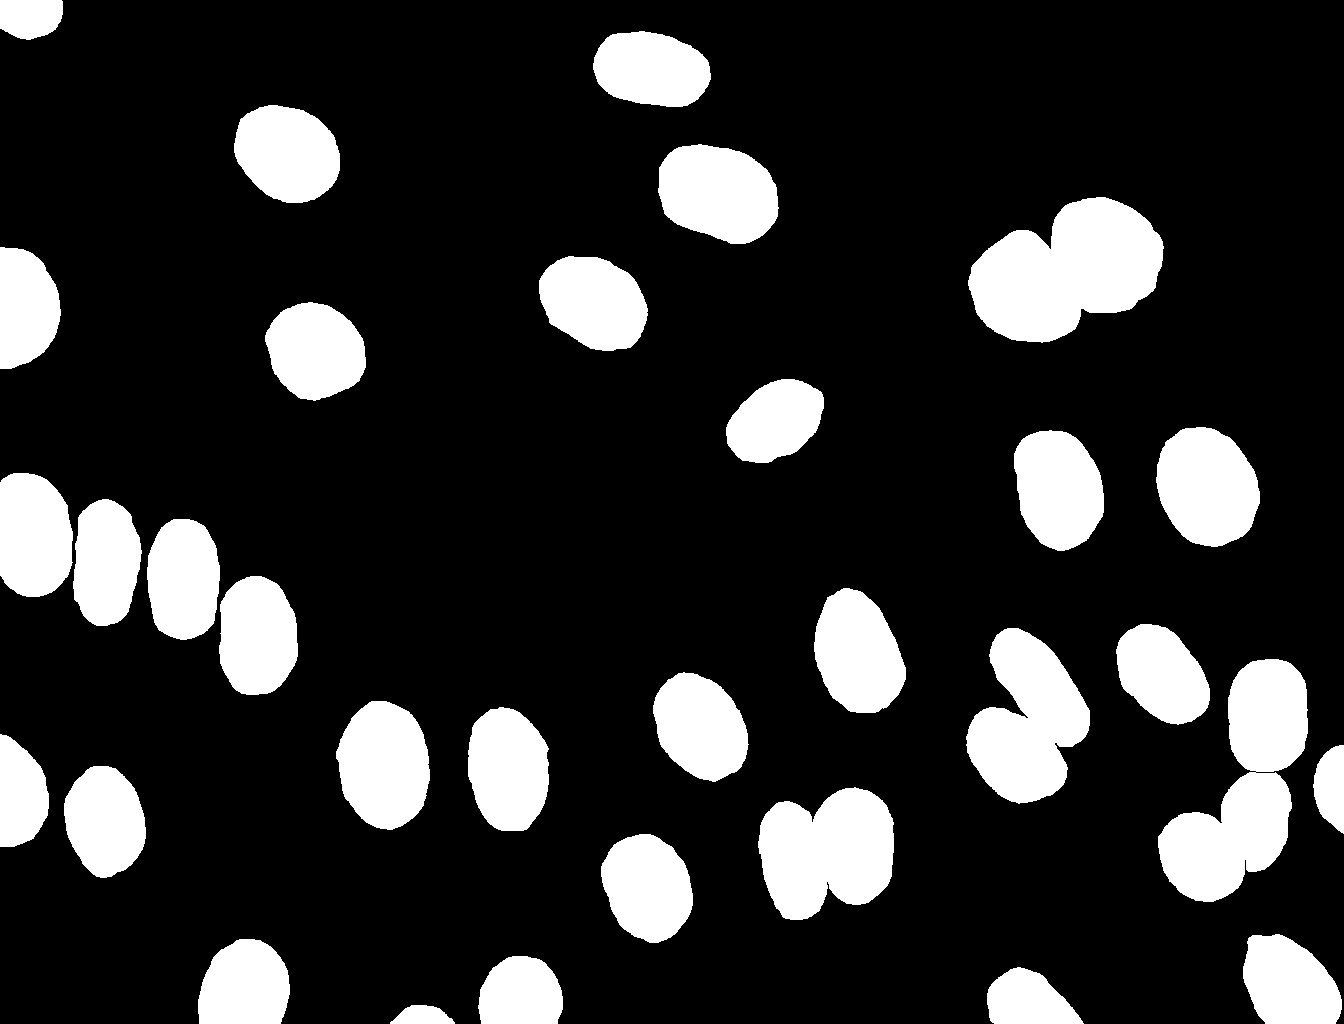
\includegraphics[width=0.5\textwidth]{images/nih3t3-im00-bingt.png}
            \caption{Segmentation ground truth for the image \texttt{data/NIH3T3/im/dna-0.png}.}
            \label{fig:nih3t3-im00-bingt}
        \end{figure}
        
        \begin{samepage}
        \item Binarize the loaded image by applying \textbf{intensity thresholding}. Adjust the threshold such that your result looks similar to Figure~\ref{fig:nih3t3-im00-bingt} -- \textbf{Hints:}
        \begin{enumerate}
            \item When working with objects of the type \texttt{numpy.ndarray} (e.g., images), mathematical operations are \emph{propagated} to the intensity values of the image. For example, if $g$ is the image \texttt{img} and $T$ is the intensity threshold \texttt{thres}, then the formal expression $g_\text{threshold}$ corresponds to ``\texttt{img >= thres}'' in Python.
            \item Exploiting propagation of mathematical expressions is \emph{faster} than writing loops. More importantly, it is also \emph{less cumbersome} and \emph{less prone to programming mistakes}. Always avoid writing loops when propagation of mathematical expressions can be used instead!
        \end{enumerate}
        \end{samepage}
        \item Evaluate your segmentation result by quantitatively comparing it to the ground truth in Figure~\ref{fig:nih3t3-im00-bingt}. Use the \textbf{Dice coefficient} for the quantitative comparison:
        \begin{gather*}
            \operatorname{Dice}\left(G, H\right) = \frac{2 \left| G \cap H \right|}{ \left|G\right| + \left|H\right|}
        \end{gather*}
        where $G$ and $H$ are the two \emph{sets of image points} corresponding to the foreground of the segmentation result (i.e.\ the binary image produced by intensity thresholding) and the foreground of the segmentation ground truth, respectively. Compute the Dice coefficient for your segmentation result -- \textbf{Hints:}
        \begin{enumerate}
            \item In Python, sets of image points are conveniently represented as \emph{binary} images (a pixel value is set to \texttt{True} if the set contains that pixel and to \texttt{False} otherwise). An image \texttt{img} is binary if \texttt{img.dtype} is \texttt{bool}.
            \item If \texttt{G} is the \emph{binary} image representing the set $G$, then \texttt{G.sum()} yields the \emph{cardinality} $\left|G\right|$ of that set.
            \item If \texttt{G} and \texttt{H} are the two \emph{binary} images representing the sets $G$ and $H$, then ``\texttt{G * H}'' yields the binary image representing $G \cap H$.
            \item Use ``\texttt{imread('../data/NIH3T3/gt/0.png')}'' to load the ground truth.
        \end{enumerate}
    \end{enumerate}
    \item Save and close the notebook. Then, shut down the notebook server.
\end{enumerate}

\begin{samepage}
\section{Sobel filter \bonustask}

As in Task~\ref{task:threshold_segm}, open the notebook \texttt{sobel.ipynb}. Extend it as follows:
\begin{enumerate}
    \item Use \texttt{imread} and \texttt{imshow} to load and show the image \texttt{../data/lena.png}.
    \item Compute the partial derivatives $g_x$ and $g_y$ by \emph{convolving} the image $g\left(x,y\right)$ with Sobel derivative operators (see Figure~\ref{fig:sobel}). To this end, implement the re-usable functions \texttt{sobel\_h} and \texttt{sobel\_v}. The functions are supposed to compute and return the \emph{convolution} of the input image \texttt{img} with the horizontal and vertical Sobel derivative operators, respectively.
    \begin{figure}[h!]
        \centering
        \raisebox{-0.8cm}{
        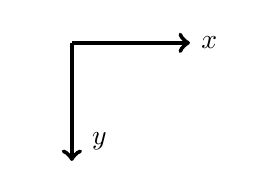
\begin{tikzpicture}
            \draw[->,ultra thick] (0,1.5)--(1.5,1.5) node[right]{$x$};
            \draw[->,ultra thick] (0,1.5)--(0.0,0.0) node[above]{\qquad$y$};
        \end{tikzpicture}}
        \qquad
        \begin{tabular}{c|>{\centering\arraybackslash}p{5mm}|>{\centering\arraybackslash}p{5mm}|>{\centering\arraybackslash}p{5mm}|}\cline{2-4}
                      & +1 & 0 & -1 \\\cline{2-4}
        $\frac{1}{8}$ & +2 & 0 & -2 \\\cline{2-4}
                      & +1 & 0 & -1 \\\cline{2-4}
        \end{tabular}
        \qquad
        \begin{tabular}{c|>{\centering\arraybackslash}p{5mm}|>{\centering\arraybackslash}p{5mm}|>{\centering\arraybackslash}p{5mm}|}\cline{2-4}
                      & +1 & +2 & +1 \\\cline{2-4}
        $\frac{1}{8}$ & \phantom{+}0 & \phantom{+}0 & \phantom{+}0 \\\cline{2-4}
                      & \laminus1 & \laminus2 & \laminus1 \\\cline{2-4}
        \end{tabular}
        \caption{Sobel derivative operators}
        \label{fig:sobel}
    \end{figure}
    \item Test your implementations for \texttt{sobel\_h} and \texttt{sobel\_v} by including images of the computed partial derivatives into your notebook (also include color legends).
    \item Compute the \emph{magnitude} of the image gradient \begin{gather*}\left\|\nabla g\left(x,y\right)\right\| = \sqrt{g_x^2\left(x,y\right) + g_y^2\left(x,y\right)}\end{gather*} and include the resulting image into the notebook. \emph{Exploit propagation of mathematical expressions instead of writing loops!}
\end{enumerate}
\end{samepage}

\end{document}
